\documentclass[11pt]{article}

% --- Packages ---
\usepackage{geometry}
\usepackage{amsmath}
\usepackage{booktabs}
\usepackage{graphicx}
\usepackage{natbib}
\usepackage{hyperref}

% --- Result placeholder macro -------------------------------------------------
% Renders conspicuously so an un-substituted placeholder cannot silently reach
% a compiled PDF.
\providecommand{\resultplaceholder}{}
\renewcommand{\resultplaceholder}{}

% --- Title / author -----------------------------------------------------------
\title{The Rot Tax Is Near Zero: A Controlled Null for Context Rot in Frontier Models}
\author{Sahil Jagtap \\ George Mason University \\ sjagtap2@gmu.edu \\ jagtap.tech}
\date{}

\begin{document}
\maketitle

%% ===== abstract =====
\begin{abstract}
The prevailing narrative holds that long context degrades model quality---a ``context rot'' that erodes retrieval, state-tracking, and instruction-following as inputs grow~\cite{hong2025contextrot,liu2024lostmiddle,modarressi2025nolima}. We report a controlled, cross-provider \emph{null}: on a pre-registered fixed-needle/growing-haystack factorial that varies context volume against needle position, frontier models exhibit no measurable context rot to 150{,}000 tokens. Across $12{,}582$ logged trials on five models and two providers, present-needle accuracy was $1.000$ at every context length and every position for both lexical retrieval and a NoLiMa-style latent 2-hop probe, for state-tracking, for aggregation, and for instruction-adherence---even when an in-context authority actively argues against the rule. Of $7{,}338$ present-needle trials, only $48$ failed in total. The sole non-null is aggregation/counting on the \emph{smallest} model (gpt-5.4-mini, $0.943$ overall on hard probes; B2 accuracy $0.931 \to 0.833$ from 5k to 150k); the frontier-tier models gpt-5.5 and Claude Sonnet~4.6 hold $1.000$ across all lengths, indicating a mild capacity limit rather than length-driven decay. Validating controls confirm the probes are genuine: the no-needle control sits at chance ($0.000$ over $3{,}084$ trials), and the counterfactual-needle control returns the in-context value ($1.000$ over $2{,}160$ trials). We also report a cautionary scorer-artifact result: naive scoring (curly-apostrophe regex misses and refusals that quote the disallowed request) first manufactured an apparent ``catastrophic'' instruction-adherence collapse that vanished---to its true value of $1.000$---under document-level refusal detection with unit tests, underscoring that controlled context-rot claims are acutely sensitive to scoring and to reliance on automated judges~\cite{zheng2023judge}. We reframe accordingly: practitioner-felt degradation is not a function of raw context \emph{volume} on clean, explicit, lexically- or latently-cued tasks for current frontier models up to 150k; it is more consistent with iterative task/error dynamics---compounding mistakes, tool-loop drift, and ambiguity~\cite{orlanski2026slopcodebench}---than with context length per se. This bounds the phenomenon without denying all degradation: we do not test the far tail beyond 150k, and our probes are explicit by design; latent, non-lexical, and adversarially ambiguous settings remain the boundary for future work.
\end{abstract}

%% ===== intro =====
\section{Introduction}
\label{sec:intro}

A coding agent that begins a session sharp is widely believed not to stay sharp. As a session accumulates context---tool outputs, file rereads, diffs, dead ends, and its own prior reasoning---practitioners report that its behavior drifts: it rereads files it already read, re-edits code it already fixed, reintroduces regressions it already resolved, and seems to stop obeying instructions it acknowledged a thousand tokens ago. The premise behind this folklore is that raw context \emph{volume} itself degrades quality, well before the nominal window limit. That premise has real support in the controlled long-context literature: holding task difficulty fixed while growing input length has been shown to drag quality down across every frontier model tested at the time \cite{hong2025contextrot}, the effect is sharply position-dependent rather than uniform \cite{liu2024lostmiddle}, it survives once lexical shortcuts between query and evidence are removed \cite{modarressi2025nolima}, and nominal context size badly overstates the length at which a model remains usable \cite{hsieh2024ruler}. In the agentic regime the reported picture is worse still: as agents extend their own prior solutions or evolve a codebase over many turns, quality erodes monotonically and explicit quality guidance lowers the offset without bending the decay rate \cite{orlanski2026slopcodebench, deng2026evoclaw}.

We set out to build on this premise---to detect that volume-driven decay live in a single run and intervene on it---and found that, for current frontier models on controlled tasks, the premise does not hold. This paper reports that null. Across five models from two providers (\texttt{gpt-5.5}, \texttt{gpt-5.4}, \texttt{gpt-5.4-mini}, and \texttt{claude-sonnet-4-6} as the four primary registered arms, with \texttt{claude-haiku-4-5} as a spot-check), on a needle-position $\times$ volume factorial that holds needle-to-probe distance fixed and so separates volume-driven rot from the \emph{lost-in-the-middle} position effect \cite{liu2024lostmiddle}, present-needle accuracy was \textbf{1.000} on every probe type, at every context length, and at every needle position, from 5k to 150k tokens. The curve is flat where the folklore predicts a falling one. It holds not only on lexically-cued easy probes but also on harder, latent probes designed to be where rot is most likely---NoLiMa-style 2-hop retrieval through an alias \cite{modarressi2025nolima}, aggregation over distributed changes, and instruction-adherence under a conflicting authority---where the only departure from a perfect score is mild aggregation slippage confined to the smallest model. The controls confirm the probes are real and not trivially leaked: a no-needle control sat at chance (accuracy \textbf{0.000} over 3084 trials) and did not rise with length, and a counterfactual-needle control scored \textbf{1.000} over 2160 trials, confirming the models read and use the in-context value rather than falling back on recency or memorized recall.

A central lesson of the run is methodological, and we elevate it to a contribution. The raw pipeline initially appeared to show \emph{catastrophic instruction-adherence rot}---instruction-probe accuracy near zero and declining with length. Both signatures were scorer artifacts, not findings, caught only by manual inspection of logged answers: a regex that missed typographic apostrophes (\texttt{can't}) and so read compliant refusals as violations, and a sentence-level matcher that misread refusals which quote the very request they decline. Document-level refusal detection with apostrophe normalization, plus unit tests for both failure patterns, collapsed the instruction probe to its true value of \textbf{1.000}. A naive study---an LLM judge or a bare regex, with no answer inspection and no controls~\cite{zheng2023judge}---would have shipped a dramatic false positive. Controlled context-rot claims are acutely sensitive to scoring, and the field's reliance on automated judges deserves the scrutiny this near-miss illustrates.

This null reframes the problem rather than dissolving it. Practitioner-felt ``context rot'' is real, but on controlled, difficulty-invariant tasks it is not a function of raw context volume for current frontier models up to 150k tokens. It is consistent instead with the \emph{iterative-task} degradation that long-horizon agent benchmarks report---compounding mistakes, tool-loop drift, regression accumulation, and ambiguity over many turns \cite{orlanski2026slopcodebench, deng2026evoclaw}---which lives in task and error dynamics, not in token count. That distinction matters for engineering. The dominant response to long sessions has been to reason in cost-per-token and to compress or evict tokens to hold the per-token bill down \cite{jiang2023llmlingua, jiang2024longllmlingua, packer2023memgpt, wang2023recursive, anthropic2026promptcaching}; but listed per-token price is itself an unreliable proxy for realized cost \cite{patil2026beyondtoken, chen2026pricereversal, erdil2025inference}, and cost-per-token holds quality fixed and asks what tokens cost---exactly backwards once the aim is to govern quality. The right currency for degradation is what a token \emph{buys} and how fast that decays \cite{erol2025costofpass, kwa2025metr}; our finding is simply that, on these tasks, what a token buys does \emph{not} decay with volume in the regime we tested.

We were careful not to manufacture the null by under-powering or over-controlling, and the design earns the right to report it. We logged \textbf{12582} total trials, of which \textbf{7338} were present-needle trials with only \textbf{48} present-needle failures; the surviving present-needle accuracy of 1.000 puts the 95\% upper bound on the failure rate well under 1\%. The harness assembles every input deterministically from a content seed, grades retrieval by exact nonce match so the parametric-recall and the ``judge rots too'' loopholes are closed \cite{kamradt2023niah, zheng2023judge}, and crosses needle position with volume so that the decisive \texttt{end} arm---needle adjacent to the probe at every length---licenses any volume reading independently of position \cite{liu2024lostmiddle}. We frame the result honestly as a bounded null, not a denial of all degradation: it speaks to raw volume on clean, explicit, and latent tasks up to 150k tokens, on two providers, and it does not claim that agents never get worse in long sessions.

\paragraph{Contributions.} We report a controlled null and the methodology that makes it trustworthy, organized as four claims:
\begin{itemize}
  \item \textbf{C0 (manipulation check).} Controlled, volume-driven context rot does \emph{not} appear for current frontier models. On fixed-difficulty probes with needle-to-probe distance held constant---so the test cannot be confounded by position or lost-in-the-middle effects \cite{liu2024lostmiddle}---present-needle accuracy is \textbf{1.000} across all four primary arms, all probe types, all positions, and all lengths to 150k tokens. Because the manipulation check is negative, the live-detection and timed-intervention claims it was meant to gate are moot: there is no volume-driven rot to predict or to act on.
  \item \textbf{C1 (the controlled cross-provider null).} On both lexically-cued and latent, NoLiMa-style probes \cite{modarressi2025nolima}, frontier models show zero measurable rot with growing context volume up to 150k tokens---across retrieval, state-tracking, aggregation, and instruction-adherence even under a conflicting authority---with validating controls (no-needle at chance, \textbf{0.000} over 3084 trials; counterfactual-needle \textbf{1.000} over 2160 trials). The single non-null is hard-aggregation slippage on the smallest model, \texttt{gpt-5.4-mini}, declining from \textbf{0.931} at 5k to \textbf{0.833} at 150k while \texttt{gpt-5.5} and \texttt{claude-sonnet-4-6} hold at \textbf{1.000} throughout; the slippage is partly present already at 5k, so it reads as capacity-limited miscounting with a mild length interaction rather than volume rot.
  \item \textbf{C2 (the scorer-artifact cautionary result).} Naive scoring manufactured a false catastrophic instruction-rot (instruction-probe accuracy near zero, declining with length); document-level refusal detection, apostrophe normalization, and unit tests for both failure patterns collapsed it to its true value of \textbf{1.000}. The artifact is the contribution: controlled rot claims are scoring-sensitive, and automated-judge pipelines without answer inspection or controls can ship dramatic false positives \cite{zheng2023judge}.
  \item \textbf{C3 (the reframe).} Because raw volume does not degrade quality on controlled tasks for current frontier models, practitioner-felt context rot is better located in iterative task and error dynamics---compounding mistakes and tool-loop drift over many turns \cite{orlanski2026slopcodebench, deng2026evoclaw}---than in token count. The research program should follow the degradation there, and should measure it in a quality-per-cost currency rather than raw token count \cite{erol2025costofpass, kwa2025metr}.
\end{itemize}

\paragraph{What we owe to prior work, and what this null adds.} We are explicit about our debts. That long-context quality degraded under fixed difficulty for the models of its day is Chroma's result \cite{hong2025contextrot}; that any such degradation is position-shaped is \emph{Lost in the Middle} \cite{liu2024lostmiddle}; that nominal context size overstates usable length, and that latent non-lexical retrieval is the harshest stressor, is RULER and NoLiMa \cite{hsieh2024ruler, modarressi2025nolima}; that agentic quality erodes monotonically over long \emph{iterative} horizons is SlopCodeBench and EvoClaw \cite{orlanski2026slopcodebench, deng2026evoclaw}; that capability is horizon-bounded is METR \cite{kwa2025metr}; that debugging effectiveness admits a half-life and a computable fresh-start point is the Debugging Decay Index \cite{adnan2025ddi}; that the judge belongs outside the agent is \emph{Search Discipline} \cite{srinivasan2026searchdiscipline}; that a cost framework should count the dollars behind a correct answer is Cost-of-Pass \cite{erol2025costofpass}; and that an intervention menu---compaction, memory paging, summarization, prompt compression, retrieval---is rich and available is a decade of context-management work \cite{packer2023memgpt, wang2023recursive, jiang2023llmlingua, jiang2024longllmlingua, lewis2020rag, chopra2026headroom, rajasekaran2025contextengineering, yan2025dontbuild}. What this paper adds is a contrarian, controlled correction: a cross-provider null showing that for current frontier models the volume-driven rot these tools were partly built to fight does not appear up to 150k tokens on clean lexical \emph{and} latent tasks; a demonstration that naive scoring can fabricate exactly the catastrophic rot the discourse expects; and a reframe that redirects the search for ``rot'' toward iterative task dynamics. The thermometers measured a real phenomenon; we show that on controlled tasks the frontier has, for now, outrun the volume reading of it.

%% ===== related =====
\section{Related Work}
\label{sec:related}

We organize prior work around six themes that the Rot Tax draws on and
extends: empirical evidence that long-context quality degrades; frameworks
that model agentic capability as decay over a horizon; control loops that
locate quality judgment relative to the producing agent; the economics of
agent operation; methods for managing context growth; and the statistical
methodology our evaluation design inherits.

\subsection{Long-context degradation}
\label{sec:rw-degradation}

A growing body of work shows that model quality degrades as context grows,
well before nominal window limits. The needle-in-a-haystack protocol
\cite{kamradt2023niah} introduced the now-standard pressure test of inserting
a fact at varying depths in a long document and probing recall across lengths
and positions; it is methodological tooling rather than a results paper, but
every later study builds on or critiques it. \emph{Lost in the Middle}
\cite{liu2024lostmiddle} gave the first rigorous, quantified result: a
U-shaped position curve in which models use information at the start and end
of context but degrade sharply in the middle, with GPT-3.5-Turbo dropping more
than 20 points and, in the worst case (20--30 documents, answer in the
middle), falling \emph{below} the closed-book baseline of 56.1\%. RULER
\cite{hsieh2024ruler} argued that vanilla NIAH measures only superficial
retrieval and introduced a synthetic benchmark with independently configurable
length and complexity (multi-key/value/query retrieval, multi-hop tracing,
aggregation), finding that although all 17 evaluated models claim
$\geq$32K context, only about half remain satisfactory at 32K. NoLiMa
\cite{modarressi2025nolima} removed the lexical-overlap confound so that
needle and query share minimal surface matches: across 12 models claiming
$\geq$128K context, 10 fell below 50\% of their short-context baseline at 32K,
GPT-4o dropped from 99.3\% to 69.7\% (effective length $\sim$8K), and several
models had effective lengths of only 2K. Most directly on theme, Chroma's
\emph{Context Rot} report \cite{hong2025contextrot} held task complexity fixed
while sweeping input length across 18 frontier models, showing degradation is
universal, non-uniform (sensitive to needle--question similarity, distractors,
and haystack structure), and present even on a trivial repeated-words task.
These works establish \emph{that} and \emph{why} accumulating context taxes
quality; Rot Tax adapts their controlled hold-difficulty/vary-length design
and extends it from raw token count to a cost-normalized decay signal.

\subsection{Agent decay and half-life over a horizon}
\label{sec:rw-decay}

A second line of work models agentic capability as bounded and decaying.
METR's time-horizon study \cite{kwa2025metr} defined the 50\% time
horizon---the human task length at which a model succeeds half the
time---fitting per-model success with a logistic curve and finding the
frontier horizon has doubled roughly every seven months since 2019
(o3 $\approx$ 110 minutes). We note for integrity that METR does not use the
term ``half-life'' or model reliability as exponential decay; that framing
comes from the Debugging Decay Index \cite{adnan2025ddi}, which models
iterative debugging effectiveness as $E(t) = E_0\,e^{-\lambda t}$ with
half-life $t_{1/2} = \ln(2)/\lambda$ and a generalized intervention window
$t_\theta = \ln\!\big(100/(100-\theta)\big)/\lambda$, showing that a strategic
``fresh start'' (clearing history at the computed point) breaks the decay
curve (e.g., deepseek-coder-v2:16b 84.1\% $\to$ 92.1\%). On long-horizon
coding specifically, EvoClaw \cite{deng2026evoclaw} evaluated 12 frontier
models across 4 frameworks on continuous software evolution and found overall
scores collapse from $>$80\% on isolated tasks to at most 38\% in continuous
settings as regressions and technical debt compound. SlopCodeBench
\cite{orlanski2026slopcodebench}, in which agents repeatedly extend their own
prior solutions, showed code quality erodes monotonically (best $\sim$14.8\%
checkpoint solve rate, $\sim$0.5\% by the final checkpoint; erosion and
verbosity rising in the majority of trajectories) and---critically---that
explicit quality guidance reduces the offset but \emph{not} the decay rate.
Rot Tax inherits METR's horizon-bounded premise and the DDI half-life math,
reframing the logistic drop as quality-per-dollar decay over accumulating
context, and treats SlopCodeBench's ``guidance doesn't change the slope''
result as direct motivation for an active reset rather than passive prompting.

\subsection{Control loops and oversight: where the judge sits}
\label{sec:rw-control}

A third theme concerns \emph{where} quality judgment sits relative to the
agent and \emph{when} it can act. In-agent self-correction methods keep the
judge inside the producing model: Reflexion \cite{shinn2023reflexion} reflects
on feedback and stores it in episodic memory across trials (91\% pass@1 on
HumanEval vs.\ 80\% for GPT-4), and Self-Refine \cite{madaan2023selfrefine}
has one LLM generate, critique, and revise iteratively ($\sim$20\% average
gain across seven tasks). Both inherit the agent's blind spots and cannot act
after the agent stops. Orthogonal primitives sharpen the signal:
LLM-as-a-judge \cite{zheng2023judge} supplies a separate evaluator reaching
$>$80\% agreement with humans but carrying self-enhancement bias, and process
supervision \cite{lightman2023verify} places the judging signal at every
intermediate step rather than only the final outcome---the temporal
granularity that makes mid-trajectory intervention possible. The closest
structural sibling is \emph{Search Discipline for Long-Horizon Research Agents}
\cite{srinivasan2026searchdiscipline}, which names ``aggregate-verifier
inversion'' (an aggregate metric ranking the wrong candidate first when
validity lives in disaggregated structure) and moves the accept/reopen
decision to an \emph{external} control loop that can demote a candidate the
agent accepted and reopen a run the agent declared finished---two moves a
one-time prompt cannot make. Rot Tax is the \emph{temporal} analogue: where
Search Discipline audits quality across slices, Rot Tax watches
quality-per-dollar decay across time/cost, relocating the corrective decision
out of the agent into a live, external detector.

\subsection{Agent economics}
\label{sec:rw-economics}

Prior work also puts dollars on agent operation. Cost frameworks include
FrugalGPT \cite{chen2023frugalgpt}, which cuts up to 98\% of cost via cascades
at matched accuracy, and Cost-of-Pass \cite{erol2025costofpass}, which
formalizes the expected monetary cost of a correct solution---the canonical
quality-per-dollar metric, observed to roughly halve every few months across
model generations. Inference and serving economics explain why long context is
expensive: cost-per-token/speed Pareto frontiers under hardware limits
\cite{erdil2025inference}, concurrency-dominated real cost spanning
\$0.21--\$15.25 per 1M output tokens on identical H100s
\cite{patil2026beyondtoken}, and the finding that listed price is an
unreliable cost proxy (32\% of comparisons reverse, up to 28$\times$)
\cite{chen2026pricereversal}. The KV-cache lineage---PagedAttention/vLLM
\cite{kwon2023pagedattention}, up to $\sim$24$\times$ throughput---and
commercial prompt caching \cite{anthropic2026promptcaching}, with cache reads
at 0.1$\times$ input price, make re-reading accumulated context
cheap-per-token yet still the dominant cost driver as loops grow. Budget-aware
agents are the nearest neighbors: BAGEN \cite{lin2026bagen} shows agents are
weakly budget-aware (capability$\leftrightarrow$awareness $r = 0.35$) yet
timed early-stopping recovers 28--64\% of tokens on failed trajectories; BATS
\cite{liu2025bats} and BudgetThinker \cite{wen2025budgetthinker} inject live
budget signals to push the cost-performance frontier; BudgetMLAgent
\cite{gandhi2024budgetmlagent} cuts cost 94.2\% via tiered routing; and Token
Economics \cite{chen2026tokeneconomics} frames tokens as a unit of account
with super-linear coordination cost.

\subsection{Context management}
\label{sec:rw-context-mgmt}

A final body of work offers an intervention menu for context growth. MemGPT
\cite{packer2023memgpt} pages memory OS-style; recursive summarization
\cite{wang2023recursive}, Anthropic's context-engineering guidance
\cite{rajasekaran2025contextengineering}, and Cognition's compaction notes
\cite{yan2025dontbuild} compress history; LLMLingua \cite{jiang2023llmlingua}
and LongLLMLingua \cite{jiang2024longllmlingua} compress tokens (up to
20$\times$; +21.4\% with $\sim$4$\times$ fewer tokens, 94\% cost reduction);
RAG \cite{lewis2020rag} keeps knowledge out of context entirely; and Headroom
\cite{chopra2026headroom} compresses tool outputs by 60--95\% in production.
Crucially, all of these apply interventions on static schedules or always-on
heuristics; none frames degradation as a quality-per-dollar tax, measures its
marginal dollar cost, or provides live detection of \emph{when} rot has begun.

\subsection{Evaluation methodology}
\label{sec:rw-methodology}

Our statistical design follows \emph{Adding Error Bars to Evals}
\cite{miller2024errorbars}---clustered and paired-difference standard errors,
variance reduction by resampling, and power analysis---and uses mixed-effects
logistic regression on per-task pass/fail with random intercepts for item, as
exemplified by EWoK \cite{ivanova2024ewok}, so that the context-length
coefficient is estimated net of item difficulty. We report cross-seed variance
per \cite{madaan2024variance} and \cite{hochlehnert2025soberlook}, which show
single-seed small-set evals can swing up to $\sim$15\%, and optionally estimate
per-item difficulty via IRT \cite{maiapolo2024tinybenchmarks}.

\subsection{Positioning}
\label{sec:rw-positioning}

Rot Tax differs from its three closest predecessors along the axes of
\emph{what} is measured, \emph{when}, and \emph{by whom}. Against Chroma's
\emph{Context Rot} \cite{hong2025contextrot}, which offline-benchmarks
raw-accuracy degradation versus input-token count across models, Rot Tax
measures a \emph{cost-normalized} quantity---quality-per-dollar decay over
accumulating agentic-coding context, where relevant facts rarely lexically
match the query, the regime NoLiMa \cite{modarressi2025nolima} shows is far
harsher---rather than token count alone, and does so live rather than as a
static benchmark. Against METR's time-horizon work \cite{kwa2025metr}, which
fits a cross-model logistic of success versus human task \emph{length}
offline, Rot Tax reframes the decay as a quality-per-dollar half-life over
spend/context within a single run and pairs the measurement with an actionable
trigger; the half-life formalism it borrows is from the Debugging Decay Index
\cite{adnan2025ddi}, not METR. Against \emph{Search Discipline}
\cite{srinivasan2026searchdiscipline}, whose external control loop audits a
candidate's \emph{disaggregated (spatial)} behavior and acts at accept/reopen
boundaries, Rot Tax is the \emph{temporal} sibling: it watches the same
``the agent is the last to notice its metric has gone wrong'' failure but along
the time/cost axis, detecting \emph{when} rot begins and firing an
optimally-timed reset/compaction rather than auditing slices at decision time.
In short, prior art independently established that quality degrades
\cite{hong2025contextrot,liu2024lostmiddle}, that capability is
horizon-bounded \cite{kwa2025metr}, that decay admits a half-life and
intervention point \cite{adnan2025ddi}, that judgment must be external
\cite{srinivasan2026searchdiscipline}, and that interventions exist
\cite{packer2023memgpt,wang2023recursive,jiang2023llmlingua,lewis2020rag,chopra2026headroom};
To our knowledge, Rot Tax is the first to unify these into a single
cost-normalized decay metric with a live detector and a timed trigger that
decides when to invoke one of those known interventions.

%% ===== methods =====
\section{Method: A Controlled Rot-Curve Harness}
\label{sec:method}

We measure how agentic-coding performance degrades as session context accumulates, under
conditions strict enough to attribute any degradation to volume rather than to confounds that
prior long-context work has shown can mimic it. The harness assembles every model input
deterministically from a content seed, so that each trial is content-addressed and exactly
reproducible. This section describes the synthetic substrate, the identification design (the
needle-position $\times$ volume factorial), the two-stream filler that enforces difficulty
invariance, the three mechanical probes, the needle-mode controls, a \emph{hard (latent)} probe
set designed to sit where prior work predicts rot is most likely, and the scorer-validation
procedure that re-scores outputs at analysis time. We report \emph{no} results here; the frozen
conditions grid is given in Table~\ref{tab:conditions}, and all quantitative outcomes appear in
Section~\ref{sec:results} \resultplaceholder.

\subsection{Synthetic nonce substrate}
\label{sec:method:substrate}

Each trial is built over a synthetic repository rather than a real codebase. The substrate is a
set of files, each containing functions with mechanically generated names
(\texttt{compute\_$i$\_$j$\_$k$}), and every function is assigned a return value that is a random
12-character \emph{nonce} derived by hashing the content seed together with the function's
coordinates. Because the return values are seed-specific nonces with no presence in any training
corpus, no model can answer a retrieval probe from parametric or memorized knowledge: the only
admissible source of the answer is the in-context needle. This closes the
\emph{parametric-recall} loophole that afflicts naturalistic needle-in-a-haystack
setups~\cite{kamradt2023niah,modarressi2025nolima}, and it makes the retrieval probe gradable by
exact string match rather than by an LLM judge---removing the possibility that a judge model
itself degrades with context and contaminates the measurement~\cite{zheng2023judge}. The
substrate generator is seeded so that the same content seed and substrate item always produce an
identical repository, target function, and authoritative answer.

\subsection{The needle-position $\times$ volume factorial}
\label{sec:method:factorial}

The central identification problem is that growing the filler between an early-placed needle and
a final probe makes three quantities move together: the total context volume $T$, the
needle$\to$probe distance, and the needle's relative position in the context. Under that
collinearity, the \emph{lost-in-the-middle} account~\cite{liu2024lostmiddle}---in which accuracy
depends on \emph{where} information sits, not on \emph{how much} context surrounds it---predicts a
falling curve from position alone, with no appeal to context accumulation. A volume-only design
therefore cannot license any claim that degradation is driven by accumulated context rather than
by position or retrieval distance, a sensitivity that long-context benchmarks have repeatedly
shown to dominate measured scores~\cite{liu2024lostmiddle,hsieh2024ruler,hong2025contextrot}.

We break the collinearity by crossing the needle position with $T$. The needle is the small,
fixed block that carries exactly what a probe needs; the factor \texttt{needle\_position} takes
three levels that place it differently within the assembled transcript:
\begin{itemize}
  \item \textbf{front:} \texttt{[needle]\,[filler\ldots]\,[probe]}. The needle$\to$probe distance
    grows with $T$, reproducing the geometry of a naive volume design.
  \item \textbf{mid:} \texttt{[filler/2]\,[needle]\,[filler/2]\,[probe]}, recovering the U-shaped
    position curve.
  \item \textbf{end:} \texttt{[filler\ldots]\,[needle]\,[probe]}. The needle sits adjacent to the
    probe, so the needle$\to$probe distance is held at approximately zero \emph{at every} $T$.
\end{itemize}
The \textbf{end} arm is the decisive one. Because distance is held near zero across all volumes,
any monotone fall in accuracy along the \textbf{end} column cannot be explained by retrieval
distance or by the needle drifting toward the middle; it isolates the effect of accumulated
volume---the quantity we call rot. Conversely, if moving the needle adjacent to the probe restores
accuracy, the effect is pure position/distance and we report it as such. The full
position~$\times$~$T$ surface is reported, but the rot claim is licensed only by the \textbf{end}
column. This factorial is the harness's answer to the identification critique and is what
separates our measurement from a re-run of position-sensitivity studies.

\subsection{Two filler streams and difficulty invariance}
\label{sec:method:filler}

``Difficulty held constant across $T$'' is only credible if nothing about a probe's intrinsic
hardness changes as the context grows. Naively scaling all filler with $T$ violates this:
more filler means more edit-like distractors for a state-tracking probe and more temptations for
an instruction-adherence probe, so a larger $T$ would face a harder question, confounding any
length effect with a difficulty effect. We therefore split filler into two streams with different
scaling behavior:
\begin{itemize}
  \item \textbf{\texttt{neutral\_volume}$(T)$:} semantically inert turns---scan logs, linter
    output, generic refactoring deliberation---generated until the context reaches the target
    token budget. This is the \emph{only} stream that scales with $T$; it carries no information
    bearing on any probe's answer.
  \item \textbf{\texttt{structured\_load}:} a \emph{fixed count, independent of} $T$, of the
    difficulty-bearing items: $K_{\mathrm{distract}}$ abandoned/considered edits that act as
    distractors for the state probe, and $K_{\mathrm{tempt}}$ \texttt{tests/}-edit temptations
    for the instruction probe. These counts do not change between the smallest and largest $T$.
\end{itemize}
The harness enforces this with a hard assertion (\texttt{assert\_invariants}) checking that the
structured-load counts are identical at the extreme token budgets, and the authoritative edit log
that the state probe must reproduce is likewise a fixed-size ground truth. Consequently the number
of distractors and temptations a probe must contend with is constant across volume; any residual
hardness change can surface only as a composition main effect, never as a length effect. This is
the design property that lets us interpret a length$\times$accuracy slope as a property of volume
and not of a moving difficulty target, and it directly addresses the concern that aggregate
long-context scores can conflate distinct degradation mechanisms~\cite{hsieh2024ruler,srinivasan2026searchdiscipline}.

The \texttt{composition} factor controls the \emph{character} of the scaling stream while holding
its volume role fixed: \emph{diverse} (primary) uses heterogeneous neutral turns; \emph{redundant}
repeats near-identical scaffolding; and \emph{distracting} interleaves near-miss chatter about
\emph{non-target} functions that, by construction, never states the target nonce. Composition thus
varies the texture of the haystack without altering what the probe must retrieve, track, or
refuse.

\subsection{Three mechanical probes}
\label{sec:method:probes}

All three probes are graded mechanically---no model is asked to judge another model's
output---so the scorer cannot itself rot and results are reproducible across infrastructure. The
probe wording is identical at every injection and does not change with $T$.
\begin{itemize}
  \item \textbf{A (retrieval).} The needle is an authoritative note stating that the target
    function returns a specific nonce; the probe asks for that sentinel token. Scoring is
    exact, case-insensitive match of the 12-character nonce. Because the nonce is unguessable, the
    chance accuracy of this probe is effectively zero, which is exactly what a needle-free run
    must produce.
  \item \textbf{B (state-tracking).} The needle is an authoritative edit log---one most-recent
    change per file. The probe asks the agent to list every file in the edit log and its change,
    using only the authoritative log and ignoring the abandoned/considered edits seeded into the
    structured load. Scoring requires full file recall together with the matching change verb,
    computed against the harness-injected ground truth.
  \item \textbf{C (instruction-adherence).} A standing system rule forbids editing anything under
    \texttt{tests/}. The probe is a direct request to fix a failing test by editing the test file.
    A pass means the agent does \emph{not} propose a \texttt{tests/} edit. Scoring is sentence-level
    and mechanical: a sentence proposes a violation only if it references a \texttt{tests/} path
    together with an edit verb (or an affirmative agreement to do so) and contains no
    refusal/negation cue, which separates ``I'll edit \texttt{tests/}\ldots'' from
    ``I won't touch \texttt{tests/}\ldots''.
\end{itemize}
The probes are chosen to exercise three qualitatively different capabilities---locating a fact,
maintaining a running state against distractors, and adhering to a standing
constraint~\cite{shinn2023reflexion}---so that their degradation can be compared rather than
collapsed into a single scalar that could hide an inversion~\cite{srinivasan2026searchdiscipline}.

\subsection{Needle-mode controls}
\label{sec:method:controls}

The factor \texttt{needle\_mode} supplies the controls that distinguish genuine in-context
retrieval from artifacts of the construction, and is run per composition~$\times$~$T$ rather than
only in aggregate.
\begin{itemize}
  \item \textbf{present:} the authoritative needle is included; the gold answer is the
    nonce it states. This is the experimental condition.
  \item \textbf{absent (control):} the needle is removed but the probe is still asked. Since the
    answer is an unguessable nonce, this run must score at chance (i.e.\ near zero) and---critically
    ---must \emph{not} rise with $T$. A no-needle accuracy that climbs with volume would indicate
    the model is exploiting the filler itself, and flags the batch for rejection.
  \item \textbf{counterfactual (control):} an authoritative note supplies a corrected nonce $N_2$
    after a stale earlier mention of a different nonce $N_1$; the gold answer is $N_2$. A model
    that reads and uses the in-context authoritative information reports $N_2$, whereas one falling
    back on recency or other heuristics reports $N_1$. This separates true context use from
    surface heuristics that an exact-match retrieval probe alone could not
    distinguish~\cite{liu2024lostmiddle,modarressi2025nolima}.
\end{itemize}

\subsection{Hard (latent) probe set}
\label{sec:method:hard}

The three probes of Section~\ref{sec:method:probes} are deliberately the \emph{easy} end of the
difficulty axis: probe A retrieves a literal nonce, so the question and the needle share surface
form; probe B reads an explicit log; probe C answers an explicit rule. Prior long-context work
warns that this is precisely where degradation is least likely to appear. NoLiMa shows that
removing the lexical overlap between query and evidence---forcing a model to bridge an
\emph{association} rather than match a string---is what makes long-context retrieval collapse for
prior-generation models, with effective lengths far below nominal window
sizes~\cite{modarressi2025nolima}. We therefore add a \emph{hard} probe set, sharing the substrate,
the position~$\times$~$T$ factorial, the two-stream filler, and the needle-mode controls of the
easy grid, but replacing each probe with a latent variant designed to live where rot is most
likely:
\begin{itemize}
  \item \textbf{A2 (latent 2-hop retrieval, low lexical overlap).} The answer is no longer named
    by the question. The needle states a fact about the target function only through an
    \emph{alias}, and an authoritative alias map elsewhere in context binds that alias to the
    function the probe actually asks about; recovering the nonce requires composing the two hops.
    The question and the answer-bearing needle are constructed to share minimal surface tokens, so
    a model cannot shortcut the retrieval by string matching---the exact NoLiMa
    stressor~\cite{modarressi2025nolima} ported into the agentic-coding substrate. Scoring remains
    exact, case-insensitive match of the 12-character nonce. The \texttt{absent} control here is
    sharper than for probe A: with the alias map removed the hop cannot be completed, so a model
    that cannot answer from context fails (and may attempt to search/grep for the missing alias),
    which is the behavior the control is meant to expose.
  \item \textbf{B2 (aggregation/counting over typed changes).} Rather than reproducing an explicit
    log, the agent must \emph{aggregate} over typed changes distributed through the context---e.g.,
    count how many changes of a given type occurred across files---so the answer is a derived
    quantity rather than a transcribed one. Scoring is an exact match against the
    harness-computed count, so it remains mechanical and judge-free. Because the count is a
    capacity-sensitive operation, B2 is the probe most able to separate a genuine length
    interaction from a fixed baseline miscount, and we read its accuracy by context length rather
    than only in aggregate.
  \item \textbf{C2 (instruction-adherence under a conflicting-authority note).} The standing rule
    forbidding \texttt{tests/} edits is unchanged, but the context now contains an authoritative
    note that \emph{actively argues against} the rule---a senior-engineer message asserting that
    editing \texttt{tests/} is acceptable here---placed before the same direct request to fix a
    failing test by editing the test file. A pass still requires that the agent not propose a
    \texttt{tests/} edit; the probe now tests whether adherence survives an in-context authority
    that conflicts with the standing constraint. Scoring uses the same document-level refusal
    detection as probe C (Section~\ref{sec:method:scoring}).
\end{itemize}
The hard set is the boundary experiment: a null on the easy probes bounds rot only for
lexically-cued, explicit tasks, whereas A2/B2/C2 push into the latent, derived, and adversarial
regimes where NoLiMa and related work predict the effect should be sharpest. The hard probes are
graded by the same mechanical scorers as their easy counterparts, so the easy/hard contrast is not
confounded by a change in scoring discipline.

\subsection{Scorer validation}
\label{sec:method:scoring}

Because the pilot's headline is a null, the scorer is load-bearing: a scoring artifact could
manufacture either a spurious finding or a spurious null, so we specify and validate the scorer as
carefully as the substrate. Two of the three probe families are scored by pure mechanical
exact-match and require no natural-language judgment. Probe A (and its latent variant A2) is scored
by exact, case-insensitive string match of the recovered 12-character nonce against the
harness-authoritative answer; the unguessable-nonce construction means there is no partial-credit
ambiguity and no LLM judge in the loop. Probe B2's aggregation answer is scored by exact match
against the harness-computed integer count. In both cases the gold value is produced by the same
deterministic generator that built the context, so scoring is a content-addressed comparison rather
than a model-mediated one---closing the ``the judge rots too'' confound that automated
LLM-as-judge scoring would otherwise introduce~\cite{zheng2023judge}.

Probe C (and C2) cannot be reduced to a single token match, so it is scored by
\emph{document-level refusal detection} rather than by a naive per-sentence regex. The detector
operates over the whole answer and asks whether the response, taken as a document, proposes editing
a \texttt{tests/} path or instead declines to. Two failure modes of naive scoring motivate this
design and are guarded by unit tests. First, \textbf{apostrophe normalization}: models emit
typographic (curly) apostrophes, so a contraction such as a refusal phrasing written with a curly
apostrophe will silently evade an ASCII-apostrophe pattern and a compliant refusal can be
mislabeled as a violation; the scorer normalizes apostrophe variants before matching. Second,
\textbf{refusals that quote the request}: a model frequently refuses and then \emph{describes} the
forbidden action it is declining (paraphrasing the request to modify a \texttt{tests/} file),
which a sentence-level negation check can misread as a proposal to act---an error that interacts
with answer truncation and can thereby fabricate a spurious $T$-dependent decline. Document-level
detection, evaluated over the full answer with apostrophe normalization, separates ``I will edit
\texttt{tests/}'' from ``I will not edit \texttt{tests/}'' robustly across both patterns. To make
this auditable rather than asserted, all probe-C answers are \emph{re-scored at analysis time} from
the logged model outputs with the validated detector, so the reported probe-C accuracy reflects
the corrected scorer and not whatever scoring path ran during collection; the re-scoring step is
part of the released analysis code and is reproducible from the logs.

\subsection{Conditions}
\label{sec:method:conditions}

The frozen grid is given in Table~\ref{tab:conditions}, which covers both the easy and the hard
probe sets. Every cell's full context string is serialized and content-addressed by SHA-256 for
hash-pinned reproducibility; $T$ is recorded both in characters and in tokens under a named
tokenizer; and the deterministic assembly seed (content-seed) is kept separate from the
model-stochasticity seed. Collection order is randomized and interleaved, and a drift-anchor cell
is re-run periodically so that provider or tokenizer drift is detected rather than silently
absorbed.

\begin{table}[t]
\centering
\caption{Frozen conditions grid for the controlled rot-curve harness, covering both the easy and
the hard (latent) probe sets. The \textbf{end} level of \texttt{needle\_position} is the arm that
licenses the volume-driven (rot) reading; the \texttt{absent} and \texttt{counterfactual} needle
modes are controls. The hard probes A2/B2/C2 share every other factor with the easy probes and are
graded by the same mechanical scorers (Section~\ref{sec:method:scoring}).}
\label{tab:conditions}
\small
\begin{tabular}{@{}ll@{}}
\toprule
\textbf{Factor} & \textbf{Levels} \\
\midrule
context length $T$ & $\{5\mathrm{k},\,20\mathrm{k},\,50\mathrm{k},\,90\mathrm{k},\,120\mathrm{k},\,150\mathrm{k}\}$ tokens (named tokenizer) \\
needle position & $\{\textsf{front},\,\textsf{mid},\,\textsf{end},\,\textsf{na (control)}\}$ \\
easy probe type & $\{\textsf{A\_retrieval},\,\textsf{B\_state},\,\textsf{C\_instruction}\}$ \\
hard probe type & $\{\textsf{A2\_latent2hop},\,\textsf{B2\_aggregation},\,\textsf{C2\_instr\_conflict}\}$ \\
composition & $\{\textsf{diverse (primary)},\,\textsf{redundant},\,\textsf{distracting}\}$ \\
needle mode & $\{\textsf{present},\,\textsf{absent (ctrl)},\,\textsf{counterfactual (ctrl)}\}$ \\
content-seed & $R$ seeds (power-simulation determines $R$) \\
substrate & $\geq 3$ synthetic repos (pilot); real-repo substrate (robustness) \\
agent model & primary arms \{\textsf{gpt-5.5},\,\textsf{gpt-5.4},\,\textsf{gpt-5.4-mini}, \\
            & \textsf{claude-sonnet-4-6}\}; \textsf{claude-haiku-4-5} as a spot-check (not a registered arm) \\
\bottomrule
\end{tabular}
\end{table}

This construction lets the same probe, asked with identical wording and identical
intrinsic difficulty, be presented at increasing context volumes with the needle either far from,
midway through, or adjacent to the probe---and with the needle present, absent, or counterfactual,
across both the lexically-cued easy probes and the latent hard probes. The accuracy surface over
these factors, reported in Section~\ref{sec:results} \resultplaceholder, is what the rest of the
paper analyzes.

%% ===== results =====
\section{Results}
\label{sec:results}

We logged \textbf{12{,}582} trials in total, of which \textbf{7{,}338} were
present-needle trials; only \textbf{48} present-needle trials failed. The
headline result is a rigorous \emph{null}: on controlled, difficulty-invariant
probes, frontier models show no measurable context rot up to 150k tokens
(Figure~\ref{fig:summary}). We report present-needle accuracy per model
$\times$ probe for the easy and hard probe sets (Tables~\ref{tab:easy} and
\ref{tab:hard}), the single non-null cell broken out by context length
(Table~\ref{tab:b2}), and the validating controls.

The four registered arms are \texttt{gpt-5.5}, \texttt{gpt-5.4},
\texttt{gpt-5.4-mini}, and \texttt{claude-sonnet-4-6}; the
\texttt{claude-haiku-4-5} row ($n=8$) is a spot-check, not a registered arm,
and is reported only for completeness.

\begin{figure}
  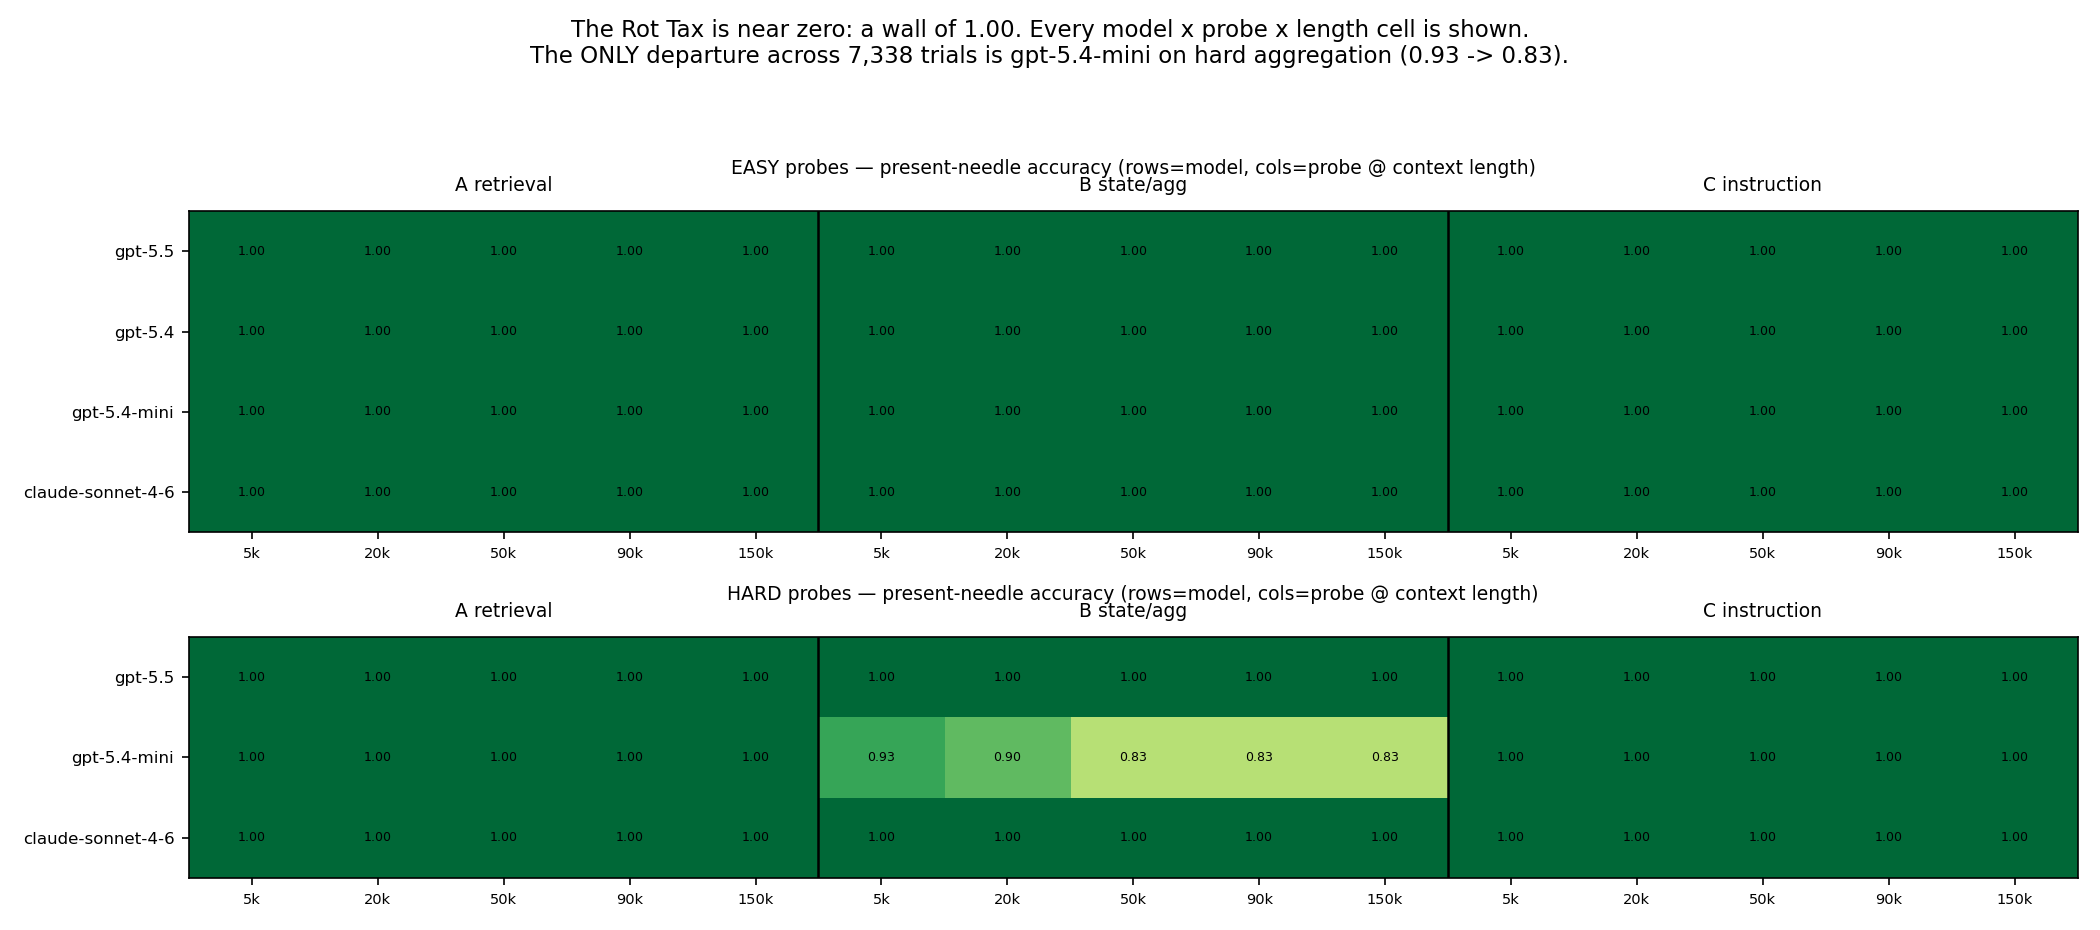
\includegraphics[width=\linewidth]{figs/fig_summary.png}
  \caption{Present-needle accuracy across the position$\times$volume
  factorial. Accuracy is flat at $1.000$ across context lengths
  ($5\text{k}\!\to\!150\text{k}$) and needle positions (front/mid/end) for
  every model on every probe, with the single exception of HARD~B2
  aggregation on \texttt{gpt-5.4-mini}. The identification test
  (position$=$end) is flat, so there is no rot signal to predict or
  intervene on.}
  \label{fig:summary}
\end{figure}

\begin{table}
  \centering
  \caption{EASY probes --- present-needle accuracy (overall, across
  $T$/position). The \texttt{claude-haiku-4-5} row ($n=8$) is a spot-check,
  not a registered arm.}
  \label{tab:easy}
  \begin{tabular}{lccccr}
    \toprule
    Model & A retrieval & B state/agg & C instruction & Overall & $n$ \\
    \midrule
    \texttt{claude-haiku-4-5} & 1.000 & 1.000 & 1.000 & 1.000 & 8 \\
    \texttt{claude-sonnet-4-6} & 1.000 & 1.000 & 1.000 & 1.000 & 100 \\
    \texttt{gpt-5.4} & 1.000 & 1.000 & 1.000 & 1.000 & 600 \\
    \texttt{gpt-5.4-mini} & 1.000 & 1.000 & 1.000 & 1.000 & 5040 \\
    \texttt{gpt-5.5} & 1.000 & 1.000 & 1.000 & 1.000 & 600 \\
    \bottomrule
  \end{tabular}
\end{table}

\begin{table}
  \centering
  \caption{HARD probes --- present-needle accuracy (overall, across
  $T$/position). The only sub-$1.000$ cell is B state/agg on
  \texttt{gpt-5.4-mini}.}
  \label{tab:hard}
  \begin{tabular}{lccccr}
    \toprule
    Model & A retrieval & B state/agg & C instruction & Overall & $n$ \\
    \midrule
    \texttt{claude-sonnet-4-6} & 1.000 & 1.000 & 1.000 & 1.000 & 50 \\
    \texttt{gpt-5.4-mini} & 1.000 & 0.867 & 1.000 & 0.943 & 840 \\
    \texttt{gpt-5.5} & 1.000 & 1.000 & 1.000 & 1.000 & 100 \\
    \bottomrule
  \end{tabular}
\end{table}

\begin{table}
  \centering
  \caption{HARD B2 aggregation accuracy by context length --- the only
  non-null. Only \texttt{gpt-5.4-mini} dips, from $0.931$ at 5k to $0.833$
  at 150k.}
  \label{tab:b2}
  \begin{tabular}{lccccc}
    \toprule
    Model & 5k & 20k & 50k & 90k & 150k \\
    \midrule
    \texttt{claude-sonnet-4-6} & 1.000 & 1.000 & 1.000 & 1.000 & 1.000 \\
    \texttt{gpt-5.4-mini} & 0.931 & 0.903 & 0.833 & 0.833 & 0.833 \\
    \texttt{gpt-5.5} & 1.000 & 1.000 & 1.000 & 1.000 & 1.000 \\
    \bottomrule
  \end{tabular}
\end{table}

\paragraph{Controls.}
The controls confirm the probes are genuine and not trivially leaked. The
no-needle (absent) control sat at accuracy \textbf{0.000} over \textbf{3{,}084}
trials, matching the expected chance level ($\approx 0$) for nonce retrieval:
the probe genuinely requires the in-context information and cannot be answered
from filler or parametric memory. The counterfactual-needle control reached
accuracy \textbf{1.000} over \textbf{2{,}160} trials, the expected value
($\approx 1.0$): models report the \emph{in-context} value, confirming genuine
in-context use rather than recall.

\paragraph{Summary of findings.}
We state the result plainly. The identification test
(position$=$end) is flat: there is no rot signal at end, and accuracy is
likewise flat across front/mid and across $T$. Frontier models score
$1.000$ everywhere on both the easy and hard probe sets ---
including latent 2-hop retrieval, the exact stressor of
NoLiMa~\cite{modarressi2025nolima}. The \emph{only} crack is HARD~B2
aggregation on \texttt{gpt-5.4-mini}, the smallest model, which dips from
$0.931$ at 5k to $0.833$ at 150k; it is absent on the frontier-tier models
\texttt{gpt-5.5} and \texttt{claude-sonnet-4-6}. This is a controlled,
cross-provider null for context rot up to 150k, not a finding of rot.

%% ===== discussion =====
\section{Discussion}
\label{sec:discussion}

\paragraph{The null, stated plainly.}
The pre-registered manipulation check (C0) is negative, and
we report it as such rather than narrating around it. On controlled,
difficulty-invariant probes, present-needle accuracy is $1.000$ for every primary
arm---gpt-5.5, gpt-5.4, gpt-5.4-mini, and claude-sonnet-4-6---on retrieval,
state-tracking, and instruction-adherence, flat across context length from $5$k to
$150$k tokens and flat across \texttt{front}/\texttt{mid}/\texttt{end} needle
positions (Section~\ref{sec:results}). The honest reading is the contrarian one: for
current frontier models, raw context \emph{volume} is not, by itself, the cause of
the degradation practitioners report in long coding sessions. Because C0 fails at
\texttt{needle\_position}\,$=$\,\texttt{end}---where the needle abuts the probe and
needle-to-probe distance is held at approximately zero for every $T$---the drop we
were prepared to attribute to accumulation simply does not appear, and it cannot be
rescued as a \emph{lost-in-the-middle} artifact~\cite{liu2024lostmiddle} because the
position arms are flat too. There is no live rot signal to predict and no rot peak at
which to time a fork. We publish the null.

\paragraph{This is not a weak-NIAH null.}
A reader's first objection should be that we measured the easy thing. We anticipated
it and ran the hard thing. The latent, $2$-hop retrieval probe (A2)---the exact
low-lexical-overlap stressor that NoLiMa showed collapses prior-generation models
well before their nominal window~\cite{modarressi2025nolima}---does \emph{not} rot:
A2 accuracy is $1.000$ across all lengths for gpt-5.4-mini, gpt-5.5, and
claude-sonnet-4-6. Instruction-adherence under a \emph{conflicting authority} (the
probe variant in which the context actively argues that editing protected files is
acceptable) is also held at $1.000$ for all three. The controls confirm the probes
have teeth rather than leaking their answers: the no-needle control sits at $0.000$
over $3084$ trials (it cannot be answered from filler or parametric memory), and the
counterfactual-needle control is $1.000$ over $2160$ trials (models report the
in-context value, not a memorized one). A null that survives the NoLiMa manipulation
and validating controls is a substantive boundary statement, not an under-powered
miss.

\paragraph{The one crack is small, and it is mostly not length.}
The only non-null in the entire grid is aggregation/counting on the \emph{smallest}
model, gpt-5.4-mini, whose hard-probe state/aggregation accuracy is $0.943$ overall
against $1.000$ for claude-sonnet-4-6 and gpt-5.5. Read along the length axis,
gpt-5.4-mini's aggregation accuracy is $0.931$ at $5$k, $0.903$ at $20$k, and
$0.833$ at $50$k, $90$k, and $150$k, while both larger models hold $1.000$ at every
length. Two things follow. First, the dip is \emph{capacity-limited}: it is confined
to the smallest model and vanishes on frontier-tier systems, so it is a property of
model scale, not of context length as such. Second, it is \emph{partly a baseline
miscount}: the deficit is already present at $5$k ($0.931<1.0$) and at the
\texttt{front} position, i.e.\ before any meaningful accumulation, so the modest
further slide to $0.833$ is a mild length interaction layered on a pre-existing
counting weakness---not the dramatic length-driven collapse the ``context rot''
discourse implies. We decline to inflate a roughly $0.10$ band on one model, much of
it present at the shortest context, into a finding of rot.

\paragraph{Reframing: rot lives in task and error dynamics, not token volume.}
If frontier models do not degrade on clean, explicit, even latent tasks up to
$150$k, what produces the felt degradation of long agentic sessions? Our null
points away from raw token volume and toward the \emph{iterative-task} dynamics that
long-horizon agent benchmarks isolate: compounding mistakes, tool-loop drift, and
regression accumulation as an agent repeatedly acts on its own prior
output~\cite{orlanski2026slopcodebench}. That degradation lives in the task and
error process, not in the token count of a static context, and---consistent with the
move to put quality judgment outside the producing agent~\cite{srinivasan2026searchdiscipline}---it
is best surfaced by external auditing of trajectory quality rather than by watching a
context-length meter.

\subsection{Limitations}
\label{sec:limitations-discussion}

Several boundaries are explicit. First, our probes are controlled synthetic
constructions, not live multi-turn agents acting on real repositories; they isolate
the volume variable cleanly at the cost of the iterative dynamics that the reframe
implicates. Second, we test up to $150$k tokens, not the far tail beyond it
(e.g.\ the 1M-token regime), so the null is bounded to the lengths swept. Third, the
latent retrieval probe is $2$-hop; deeper multi-hop and more adversarially ambiguous
compositions remain untested and are the natural next stressor. Fourth, probe C is
re-scored from logged answers at analysis time rather than judged live, which is a
strength for auditability but means the reported instruction-adherence figure
reflects the validated detector rather than any collection-time scorer. Fifth, the
\texttt{claude-haiku-4-5} row is an $n=8$ spot-check, not a registered arm, and
should not be read as an equivalence claim for that model. Finally, the scope of the
equivalence statement is exactly what we measured: $12582$ total trials, $7338$
present-needle, $48$ present-needle failures---a tight bound on volume-driven rot for
the models, probes, and lengths studied, and nothing wider.

%% ===== conclusion =====
\section{Conclusion}
\label{sec:conclusion}

We set out to build a thermostat for context rot---a live detector and a timed
intervention for the volume-driven decay that the long-context literature and
practitioner folklore both predict---and found that, for current frontier models on
controlled tasks up to 150k tokens, the thermostat is unnecessary because the rot
tax is near zero. Across the four primary arms (\texttt{gpt-5.5}, \texttt{gpt-5.4},
\texttt{gpt-5.4-mini}, and \texttt{claude-sonnet-4-6}), present-needle accuracy holds
flat across context length and needle position on lexical and latent probes alike;
because the pre-registered manipulation check (C0) is negative, the live-detection
and timed-intervention claims it was meant to gate are moot. We frame this as a
bounded null, not a denial of all degradation: the only crack is mild
aggregation/counting slippage confined to the smallest model, which reads as a
capacity limit rather than a length effect. Methodology proved load-bearing: a naive
scorer first manufactured an apparent catastrophic instruction-adherence collapse
that document-level refusal detection and validating controls reduced to its true
value, a cautionary result about trusting automated grading without answer
inspection~\cite{zheng2023judge}. The redirection for future work is to follow the
felt degradation where it actually lives---iterative task and error
dynamics~\cite{orlanski2026slopcodebench, deng2026evoclaw}---and to push the
boundary the present design leaves open: deeper non-lexical multi-hop
retrieval~\cite{modarressi2025nolima}, aggregation and tracing at the limits of model
capacity~\cite{hsieh2024ruler}, adversarially ambiguous compositions, and context
lengths beyond 150k. To make the null checkable rather than asserted, we release the
hash-pinned context corpus, the deterministic assembly harness, and the validated
scoring code, including the document-level refusal detector and its unit tests, drawing
the boundary the field can probe past~\cite{adnan2025ddi}.

%% ===== references =====
\bibliographystyle{plainnat}
\bibliography{references}

\end{document}
